\subsection{Representação final do batimento}

O vetor final reúne 18 features e altera apenas a forma de resumir o batimento
filtrado e o seu contexto rítmico local. Não há descritores do sinal bruto nem
expansão massiva de dimensionalidade. A intenção é manter um conjunto compacto,
interpretável e coerente com a segmentação ancorada no R-peak.

\begin{table*}[!htbp]
  \centering
  \caption{Grupos de features da representação final.}
  \label{tab-feature-groups}
  \scriptsize
  \renewcommand{\arraystretch}{1.08}
  \begin{tabular}{lp{8.6cm}r}
    \toprule
    Grupo & Variáveis & Quantidade \\
    \midrule
    Morfologia filtrada & amplitude em R, pico-a-pico, energia, área absoluta, inclinação máxima absoluta e desvio-padrão & 6 \\
    Ritmo & RR anterior, RR posterior e razão RR & 3 \\
    Espectrais & centroide espectral, largura de banda, potência em 8 a 20 Hz e potência em 20 a 40 Hz & 4 \\
    Gabor & energia em P, energia em QRS, máximo em QRS, deslocamento do pico em QRS e energia em T & 5 \\
    \bottomrule
  \end{tabular}
  \renewcommand{\arraystretch}{1.0}
\end{table*}

As features morfológicas resumem amplitude, energia, área absoluta,
variabilidade e inclinação máxima do batimento filtrado. As features rítmicas
capturam o contexto local do intervalo RR antes e depois da batida. Os
descritores espectrais medem quão concentrada ou espalhada está a energia da
janela, com ênfase nas bandas de 8 a 20 Hz e 20 a 40 Hz, associadas a
componentes mais rápidas do QRS. Esse desenho mantém a comparação no domínio do
sinal tratado por DSP e explicita que o vetor final usa morfologia, ritmo,
espectro e respostas locais, não amostras cruas da janela.

\subsection{Banco Gabor do notebook}

A representação final usa exatamente o banco consolidado no notebook do grupo.
A região P recebe um filtro par em 8 Hz com janela de -0,28 s a -0,07 s. A
região QRS recebe um filtro em magnitude em 15 Hz com janela de -0,07 s a
0,07 s. A região T recebe um filtro par em 6 Hz com janela de 0,18 s a 0,45 s.
A Figura~\ref{fig-gabor-bank} mostra os três kernels normalizados, e a
Figura~\ref{fig-gabor-response} ilustra as respostas alinhadas em um batimento
normal e em um batimento anômalo.

\begin{figure}[!htbp]
  \centering
  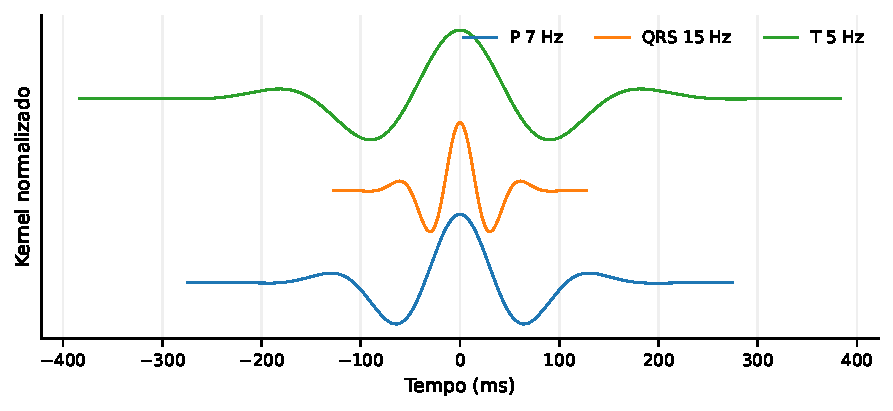
\includegraphics[width=0.95\linewidth]{figures/fig_gabor_filter_bank.pdf}
  \caption{Banco compacto de filtros Gabor 1D usado na representação final.}
  \label{fig-gabor-bank}
\end{figure}

\begin{figure}[!htbp]
  \centering
  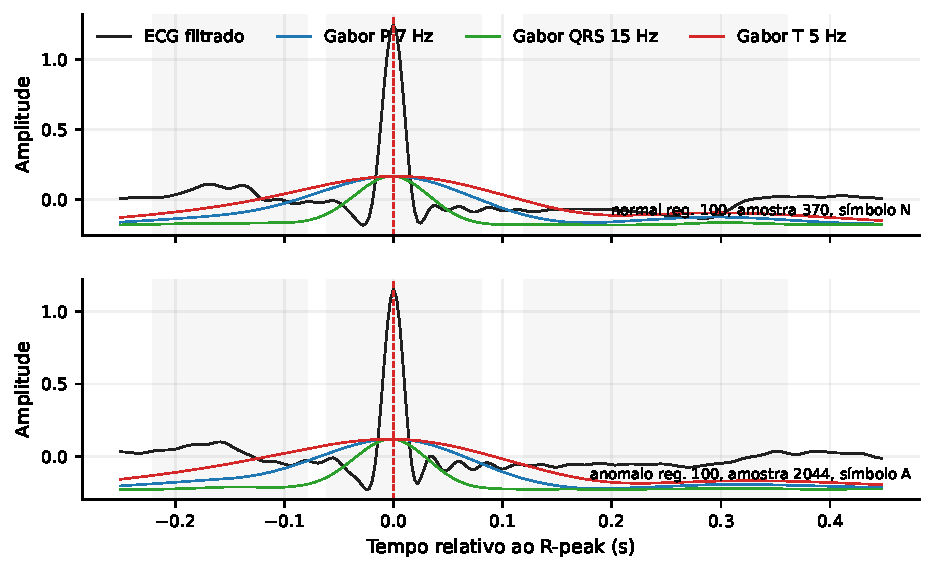
\includegraphics[width=0.95\linewidth]{figures/fig_gabor_response_examples.pdf}
  \caption{Respostas Gabor em um batimento normal e em um batimento anômalo, com janelas aproximadas de P, QRS e T destacadas.}
  \label{fig-gabor-response}
\end{figure}

\subsection{Modelos e métricas}

Dois modelos compartilham a mesma padronização das 18 features, mas usam
regimes de treinamento diferentes. A SVM supervisionada usa kernel RBF,
\texttt{class\_weight=balanced}, \texttt{gamma=scale} e probabilidades
habilitadas. Esse modelo é ajustado com todos os 51.002 batimentos do treino
DS1. A One-Class SVM usa kernel RBF, \texttt{nu=0.05} e
\texttt{gamma=scale}, sendo ajustada apenas com os 38.088 batimentos normais de
DS1.

PR-AUC é a métrica principal. ROC-AUC, precision, recall, F1 e matriz de
confusão complementam a análise. A SVM supervisionada é avaliada pelo escore de
probabilidade da classe anômala, enquanto a One-Class SVM usa o valor negativo
da \texttt{decision\_function}, orientado para que escores maiores representem
maior anomalia.

\begin{figure}[H]
  \centering
  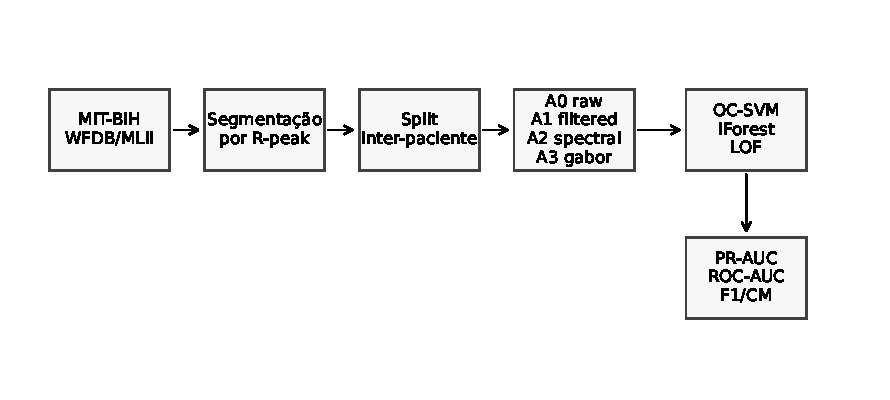
\includegraphics[width=1.0\linewidth]{figures/fig_pipeline_ablation.pdf}
  \caption{Pipeline experimental resumido.}
  \label{fig-pipeline}
\end{figure}
\FloatBarrier
